\section{Introdução}
\subsection*{Paper de 2018}
\begin{frame}{\subsecname}
    \centering
    
\includegraphics[width=\textwidth]{fig/paper.png}
\end{frame}
\subsection*{Vantagens}
\begin{frame}{\subsecname}
    \begin{itemize}
        \item<1-> Independente de parâmetros
        \item<2-> Totalmente discreto
        \item<3-> Não precisa minimizar função
    \end{itemize}
\end{frame}
\subsection*{Aplicações}
\begin{frame}{\subsecname}
    \begin{itemize}
        \item<1-> Dígitos manuscritos
        \only<1>{\begin{figure}
            \centering
            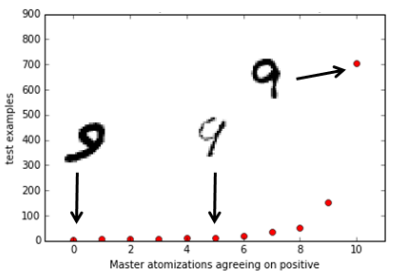
\includegraphics[scale=0.5]{fig/hand.png}
            \label{fig:hand}
        \end{figure}}
        \item<2-> N-rainhas
        \only<2>{\begin{figure}
            \centering
            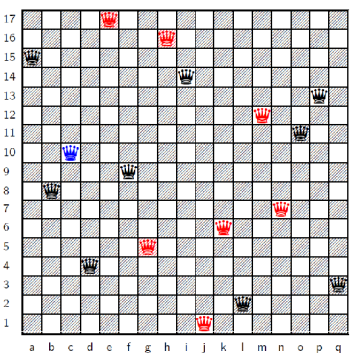
\includegraphics[scale=0.5]{fig/nrainhas.png}
            \label{fig:nrainhas}
        \end{figure}}
    \end{itemize}
\end{frame}